\let\negmedspace\undefined
\let\negthickspace\undefined
\documentclass[journal,12pt,onecolumn]{IEEEtran}
\usepackage{cite}
\usepackage{amsmath,amssymb,amsfonts,amsthm}
\usepackage{algorithmic}
\usepackage{graphicx}
\graphicspath{{./figs/}}
\usepackage{textcomp}
\usepackage{xcolor}
\usepackage{txfonts}
\usepackage{listings}
\usepackage{enumitem}
\usepackage{mathtools}
\usepackage{gensymb}
\usepackage{comment}
\usepackage{caption}
\usepackage[breaklinks=true]{hyperref}
\usepackage{tkz-euclide} 
\usepackage{listings}
\usepackage{gvv}                                        
%\def\inputGnumericTable{}                                 
\usepackage[latin1]{inputenc}     
\usepackage{xparse}
\usepackage{color}                                            
\usepackage{array}                                            
\usepackage{longtable}                                       
\usepackage{calc}                                             
\usepackage{multirow}
\usepackage{multicol}
\usepackage{hhline}                                           
\usepackage{ifthen}                                           
\usepackage{lscape}
\usepackage{tabularx}
\usepackage{array}
\usepackage{float}
\newtheorem{theorem}{Theorem}[section]
\newtheorem{problem}{Problem}
\newtheorem{proposition}{Proposition}[section]
\newtheorem{lemma}{Lemma}[section]
\newtheorem{corollary}[theorem]{Corollary}
\newtheorem{example}{Example}[section]
\newtheorem{definition}[problem]{Definition}
\newcommand{\BEQA}{\begin{eqnarray}}
\newcommand{\EEQA}{\end{eqnarray}}
\newcommand{\define}{\stackrel{\triangle}{=}}
\theoremstyle{remark}
\newtheorem{rem}{Remark}

\begin{document}
\title{
ASSIGNMENT 3: GATE 2018 \\
IN: INSTRUMENTATION ENGINEERING}
\author{EE25BTECH11062 - Vivek K Kumar}
\maketitle
\renewcommand{\thefigure}{\theenumi}
\renewcommand{\thetable}{\theenumi}

\begin{enumerate}
    \item "When she fell down the \underline{\hspace{2cm}} she received many \underline{\hspace{2cm}} but little help." 
    The words that best fill the blanks in the above sentence are
    
    \hfill{\brak{\text{GATE IN 2018}}}
    \begin{enumerate}
        \begin{multicols}{2}
            \item stairs, stares
            \item stairs, stairs
            \item stares, stairs
            \item stares, stares
        \end{multicols}
    \end{enumerate}

    \item "In spite of being warned repeatedly, he failed to correct his \underline{\hspace{2cm}} behaviour."
    The word that best fills the blank in the above sentence is
    
    \hfill{\brak{\text{GATE IN 2018}}}
    \begin{enumerate}
        \begin{multicols}{4}
            \item rational
            \item reasonable
            \item errant
            \item good
        \end{multicols}
    \end{enumerate}

    \item For $0 \le x \le 2\pi$, $\sin x$ and $\cos x$ are both decreasing functions in the interval
    
    \hfill{\brak{\text{GATE IN 2018}}}
    \begin{enumerate}
        \begin{multicols}{4}
            \item $\brak{0,\frac{\pi}{2}}$
            \item $\brak{\frac{\pi}{2},\pi}$
            \item $\brak{\pi,\frac{3\pi}{2}}$
            \item $\brak{\frac{3\pi}{2},2\pi}$
        \end{multicols}
    \end{enumerate}

    \item The area of an equilateral triangle is $\sqrt{3}$. What is the perimeter of the triangle?
    
    \hfill{\brak{\text{GATE IN 2018}}}
    \begin{enumerate}
        \begin{multicols}{4}
            \item $2$
            \item $4$
            \item $6$
            \item $8$
        \end{multicols}
    \end{enumerate}

    \item Arrange the following three-dimensional objects in the descending order of their volumes:
    \begin{itemize}
        \item \brak{i} A cuboid with dimensions $10$ cm, $8$ cm and $6$ cm
        \item \brak{ii} A cube of side $8$ cm
        \item \brak{iii} A cylinder with base radius $7$ cm and height $7$ cm
        \item \brak{iv} A sphere of radius $7$ cm
    \end{itemize}
    
    \hfill{\brak{\text{GATE IN 2018}}}
    \begin{enumerate}
        \begin{multicols}{2}
            \item \brak{i}, \brak{ii}, \brak{iii}, \brak{iv}
            \item \brak{ii}, \brak{i}, \brak{iv}, \brak{iii}
            \item \brak{iii}, \brak{ii}, \brak{i}, \brak{iv}
            \item \brak{iv}, \brak{iii}, \brak{ii}, \brak{i}
        \end{multicols}
    \end{enumerate}

    \item An automobile travels from city A to city B and returns to city A by the same route. The speed of the vehicle during the onward and return journeys were constant at $60$ km/h and $90$ km/h respectively. What is the average speed in km/h for the entire journey?
    
    \hfill{\brak{\text{GATE IN 2018}}}
    \begin{enumerate}
        \begin{multicols}{4}
            \item $72$
            \item $73$
            \item $74$
            \item $75$
        \end{multicols}
    \end{enumerate}

    \item A set of $4$ parallel lines intersect with another set of $5$ parallel lines. How many parallelograms are formed?
    
    \hfill{\brak{\text{GATE IN 2018}}}
    \begin{enumerate}
        \begin{multicols}{4}
            \item $20$
            \item $48$
            \item $60$
            \item $72$
        \end{multicols}
    \end{enumerate}
    
    \item To pass a test, a candidate needs to answer at least $2$ out of $3$ questions correctly. A total of $6,30,000$ candidates appeared for the test. Question A was correctly answered by $3,30,000$ candidates. Question B was answered correctly by $2,50,000$ candidates. Question C was answered correctly by $2,60,000$ candidates. Both questions A and B were answered correctly by $1,00,000$ candidates. Both questions B and C were answered correctly by $90,000$ candidates. Both questions A and C were answered correctly by $80,000$ candidates. If the number of students answering all questions correctly is the same as the number answering none, how many candidates failed to clear the test?
    
    \hfill{\brak{\text{GATE IN 2018}}}
    \begin{enumerate}
        \begin{multicols}{4}
            \item $30,000$
            \item $2,70,000$
            \item $3,90,000$
            \item $4,20,000$
        \end{multicols}
    \end{enumerate}

    \item If $x^{2}+x-1=0$ what is the value of $x^{4}+\frac{1}{x^{4}}$?
    
    \hfill{\brak{\text{GATE IN 2018}}}
    \begin{enumerate}
        \begin{multicols}{4}
            \item $1$
            \item $5$
            \item $7$
            \item $9$
        \end{multicols}
    \end{enumerate}
    
    \item In a detailed study of annual crow births in India, it was found that there was relatively no growth during the period $2002$ to $2004$ and a sudden spike from $2004$ to $2005$. In another unrelated study, it was found that the revenue from cracker sales in India which remained fairly flat from $2002$ to $2004$, saw a sudden spike in $2005$ before declining again in $2006$. The solid line in the graph below refers to annual sale of crackers and the dashed line refers to the annual crow births in India. Choose the most appropriate inference from the above data.
    \begin{figure}[H]
        \centering
        \includegraphics[width=0.6\columnwidth]{q10.png}
        \caption*{}
        \label{fig:q10}
    \end{figure}
    
    \hfill{\brak{\text{GATE IN 2018}}}
    \begin{enumerate}
        \item There is a strong correlation between crow birth and cracker sales.
        \item Cracker usage increases crow birth rate.
        \item If cracker sale declines, crow birth will decline.
        \item Increased birth rate of crows will cause an increase in the sale of crackers.
    \end{enumerate}

\end{enumerate}

\begin{enumerate}
    \item Let N be a $3$ by $3$ matrix with real number entries. The matrix N is such that $N^{2}=0$. The eigenvalues of N are
    
    \hfill{\brak{\text{GATE IN 2018}}}
    \begin{enumerate}
        \begin{multicols}{4}
            \item $0,0,0$
            \item $0,0,1$
            \item $0,1,1$
            \item $1,1,1$
        \end{multicols}
    \end{enumerate}

    \item Let $f_{1}\brak{z}=z^{2}$ and $f_{2}\brak{z}=\overline{z}$ be two complex variable functions. Here $\overline{z}$ is the complex conjugate of z. Choose the correct answer.
    
    \hfill{\brak{\text{GATE IN 2018}}}
    \begin{enumerate}
        \item Both $f_{1}\brak{z}$ and $f_{2}\brak{z}$ are analytic
        \item Only $f_{1}\brak{z}$ is analytic
        \item Only $f_{2}\brak{z}$ is analytic
        \item Both $f_{1}\brak{z}$ and $f_{2}\brak{z}$ are not analytic
    \end{enumerate}
    
    \item X and Y are two independent random variables with variances $1$ and $2$, respectively. Let $Z=X-Y$. The variance of Z is
    
    \hfill{\brak{\text{GATE IN 2018}}}
    \begin{enumerate}
        \begin{multicols}{4}
            \item $0$
            \item $1$
            \item $2$
            \item $3$
        \end{multicols}
    \end{enumerate}
    
    \item Consider two functions $f\brak{x}=\brak{x-2}^{2}$ and $g\brak{x}=2x-1$, where x is real. The smallest value of x for which $f\brak{x}=g\brak{x}$ is \underline{\hspace{2cm}}.
    
    \hfill{\brak{\text{GATE IN 2018}}}
    
    \item Consider a sequence of tossing of a fair coin where the outcomes of tosses are independent. The probability of getting the head for the third time in the fifth toss is
    
    \hfill{\brak{\text{GATE IN 2018}}}
    \begin{enumerate}
        \begin{multicols}{4}
            \item $\frac{5}{16}$
            \item $\frac{3}{16}$
            \item $\frac{3}{5}$
            \item $\frac{9}{16}$
        \end{multicols}
    \end{enumerate}
    
    \item A series R-C circuit is excited by a $1\angle0$ V sinusoidal ac voltage source. The locus diagram of the phasor current $I=\brak{x+jy}$ A, when C is varied, while keeping R fixed, is
    
    \hfill{\brak{\text{GATE IN 2018}}}
    \begin{enumerate}
    \begin{figure}[H]
    \centering
        \begin{multicols}{2}
            \item \includegraphics[width=0.5\columnwidth]{q6a.png}
            \item \includegraphics[width=0.5\columnwidth]{q6b.png}
            \item \includegraphics[width=0.5\columnwidth]{q6c.png}
            \item \includegraphics[width=0.5\columnwidth]{q6d.png}
        \end{multicols}
        \caption*{} 
        \label{fig:q6} 
        \end{figure}
    \end{enumerate}

    \item The Thevenin equivalent circuit representation across terminals $p-q$ of the circuit shown in the figure is a
    \begin{figure}[H]
        \centering
        \includegraphics[width=0.5\columnwidth]{q7.png}
        \caption*{}
        \label{fig:q7}
    \end{figure}
    
    \hfill{\brak{\text{GATE IN 2018}}}
    \begin{enumerate}
        \begin{multicols}{2}
            \item $1$ V source in series with $150$ k$\ohm$
            \item $1$ V source in parallel with $100$ k$\ohm$
            \item $2$ V source in series with $150$ k$\ohm$
            \item $2$ V source in parallel with $200$ k$\ohm$
        \end{multicols}
    \end{enumerate}

    \item A coil having an impedance of $\brak{10+j100}$ $\ohm$ is connected in parallel to a variable capacitor as shown in figure. Keeping the excitation frequency unchanged, the value of the capacitor is changed so that parallel resonance occurs. The impedance across terminals p-q at resonance \brak{\text{in } \ohm} is \underline{\hspace{2cm}}.
    \begin{figure}[H]
        \centering
        \includegraphics[width=0.3\columnwidth]{q8.png}
        \caption*{}
        \label{fig:q8}
    \end{figure}
    
    \hfill{\brak{\text{GATE IN 2018}}}
    
    \item Two periodic signals $x\brak{t}$ and $y\brak{t}$ have the same fundamental period of $3$ seconds. Consider the signal $z\brak{t}=x\brak{-t}+y\brak{2t+1}$. The fundamental period of $z\brak{t}$ in seconds is
    
    \hfill{\brak{\text{GATE IN 2018}}}
    \begin{enumerate}
        \begin{multicols}{4}
            \item $1$
            \item $1.5$
            \item $2$
            \item $3$
        \end{multicols}
    \end{enumerate}

    \item Consider signal $x\brak{t}=\begin{cases}1, & \abs{t} \le 2\\ 0, & \abs{t}>2\end{cases}$. Let $\delta\brak{t}$ denote the unit impulse \brak{Dirac-delta} function. The value of the integral $\int_{0}^{5}2x\brak{t-3}\delta\brak{t-4}dt$ is
    
    \hfill{\brak{\text{GATE IN 2018}}}
    \begin{enumerate}
        \begin{multicols}{4}
            \item $2$
            \item $1$
            \item $0$
            \item $3$
        \end{multicols}
    \end{enumerate}

    \item An ideal square wave with period of $20$ ms shown in the figure, is passed through an ideal low pass filter with cut-off frequency $120$ Hz. Which of the following is an accurate description of the output?
    \begin{figure}[H]
        \centering
        \includegraphics[width=0.8\columnwidth]{q11.png}
        \caption*{}
        \label{fig:q11}
    \end{figure}
    
    \hfill{\brak{\text{GATE IN 2018}}}
    \begin{enumerate}
        \item Output is zero.
        \item Output consists of both $50$ Hz and $100$ Hz frequency components.
        \item Output is a pure sinusoid of frequency $50$ Hz.
        \item Output is a square wave of fundamental frequency $50$ Hz.
    \end{enumerate}

    \item An input $p\brak{t}=\sin\brak{t}$ is applied to the system $G\brak{s}=\frac{s-1}{s+1}$. The corresponding steady state output is $y\brak{t}=\sin\brak{t+\varphi}$, where the phase $\varphi$ \brak{\text{in degrees}}, when restricted to $0\degree\le\varphi\le360\degree$ is \underline{\hspace{2cm}}.
    
    \hfill{\brak{\text{GATE IN 2018}}}
    
    \item The approximate phase response of $\frac{100^{2}e^{-0.01~s}}{s^{2}+0.2~s+100^{2}}$ is
    
    \hfill{\brak{\text{GATE IN 2018}}}
    \begin{enumerate}
    \begin{figure}[H]
        \begin{multicols}{2}
            \item \includegraphics[width=0.9\columnwidth]{q13a.png}
            \item \includegraphics[width=0.9\columnwidth]{q13b.png}
            \item \includegraphics[width=0.9\columnwidth]{q13c.png}
            \item \includegraphics[width=0.9\columnwidth]{q13d.png}
        \end{multicols}
         \caption*{} 
         \label{fig:q13} 
        \end{figure}
    \end{enumerate}

    \item Consider the transfer function $G\brak{s}=\frac{2}{\brak{s+1}\brak{s+2}}$. The phase margin of $G\brak{s}$ in degrees is \underline{\hspace{2cm}}.
    
    \hfill{\brak{\text{GATE IN 2018}}}

    
    \item In the given circuit, assume that the opamp is ideal and the transistor has a $\beta$ of $20$. The current $I_{o}$ \brak{\text{in }mu\text{A}} flowing through the load $Z_{L}$ is \underline{\hspace{2cm}}.
    \begin{figure}[H]
        \centering
        \includegraphics[width=0.4\columnwidth]{q15.png}
        \caption*{}
        \label{fig:q15}
    \end{figure}
    
    \hfill{\brak{\text{GATE IN 2018}}}
    
    \item The diodes given in the circuit are ideal. At $t=60$ ms, $V_{pq}$ \brak{\text{in Volts}} is \underline{\hspace{2cm}}.
    \begin{figure}[H]
        \centering
        \includegraphics[width=0.5\columnwidth]{q16.png}
        \caption*{}
        \label{fig:q16}
    \end{figure}
    
    \hfill{\brak{\text{GATE IN 2018}}}

    \item For the 3-bit binary counter shown in the figure, the output increments at every positive transition in the clock \brak{CLK}. Assume ideal diodes and the starting state of the counter as $000$. If output high is $1$ V and output low is $0$ V, the current I \brak{\text{in mA}} flowing through the $50~\ohm$ resistor during the $5^{th}$ clock cycle is \brak{\text{up to one decimal place}} \underline{\hspace{2cm}}.
    \begin{figure}[H]
        \centering
        \includegraphics[width=0.6\columnwidth]{q17.png}
        \caption*{}
        \label{fig:q17}
    \end{figure}
    
    \hfill{\brak{\text{GATE IN 2018}}}
    
    \item The representation of the decimal number $\brak{27.625}_{10}$ in base-2 number system is
    
    \hfill{\brak{\text{GATE IN 2018}}}
    \begin{enumerate}
        \begin{multicols}{2}
            \item $11011.110$
            \item $11101.101$
            \item $11011.101$
            \item $10111.110$
        \end{multicols}
    \end{enumerate}

    \item The number of comparators required for implementing an 8-bit flash analog-to-digital converter is
    
    \hfill{\brak{\text{GATE IN 2018}}}
    \begin{enumerate}
        \begin{multicols}{4}
            \item $8$
            \item $128$
            \item $255$
            \item $256$
        \end{multicols}
    \end{enumerate}

    \item A voltage of $6\cos\brak{100\pi t}$ V is fed as y-input to a CRO. The waveform seen on the screen of the CRO is shown in the figure. The Y and X axes settings for the CRO are respectively
    \begin{figure}[H]
        \centering
        \includegraphics[width=0.6\columnwidth]{q20.png}
        \caption*{}
        \label{fig:q20}
    \end{figure}
    
    \hfill{\brak{\text{GATE IN 2018}}}
    \begin{enumerate}
        \begin{multicols}{2}
            \item $1$ V/div and $1$ ms/div
            \item $1$ V/div and $2$ ms/div
            \item $2$ V/div and $1$ ms/div
            \item $2$ V/div and $2$ ms/div
        \end{multicols}
    \end{enumerate}

    \item A $300$ V, $5$A, $0.2$ pf low power factor wattmeter is used to measure the power consumed by a load. The wattmeter scale has $150$ divisions and the pointer is on the $100^{th}$ division. The power consumed by the load \brak{\text{in Watts}} is \underline{\hspace{2cm}}.
    
    \hfill{\brak{\text{GATE IN 2018}}}

    \item As shown in the figure, temperature $\theta$ is measured using a K type thermocouple. It has a sensitivity of $40~\mu V/\degree C$. The gain \brak{\text{G}} of the ideal instrumentation amplifier is $25$. If the output $V_{o}$ is $96$ mV, then the value of $\theta$ \brak{\text{in }\degree\text{C}} is \underline{\hspace{2cm}}.
    \begin{figure}[H]
        \centering
        \includegraphics[width=0.6\columnwidth]{q22.png}
        \caption*{}
        \label{fig:q22}
    \end{figure}
    
    \hfill{\brak{\text{GATE IN 2018}}}

    \item A piezoelectric pressure sensor has a bandpass characteristic with cut-off frequencies of $0.1$ Hz and $1$ MHz, and a sensitivity of $100$ mV/kPa. The sensor is subjected to a static constant pressure of $100$ kPa. Its steady-state output will be
    
    \hfill{\brak{\text{GATE IN 2018}}}
    \begin{enumerate}
    \begin{multicols}{4}
        \item $0$ V
        \item $0.1$ V
        \item $1$ V
        \item $10$ V
    \end{multicols}
    \end{enumerate}

    \item An amplitude modulated signal is shown in the figure. The modulation index is \brak{\text{up to one decimal place}} \underline{\hspace{2cm}}.
    \begin{figure}[H]
        \centering
        \includegraphics[width=0.5\columnwidth]{q24.png}
        \caption*{}
        \label{fig:q24}
    \end{figure}
    
    \hfill{\brak{\text{GATE IN 2018}}}

    \item An optical pulse containing $6\times10^{6}$ photons is incident on a photodiode and $4.5\times10^{6}$ electron-hole pairs are created. The maximum possible quantum efficiency \brak{\text{in }\%} of the photodiode is \underline{\hspace{2cm}}.
    
    \hfill{\brak{\text{GATE IN 2018}}}
    
    \item Given $\vec{F}=\brak{x^{2}-2y}\vec{i}-4yz\vec{j}+4xz^{2}\vec{k}$, the value of the line integral $\int_{c}\vec{F}\cdot d\vec{l}$ along the straight line c from $\brak{0,0,0}$ to $\brak{1,1,1}$ is
    
    \hfill{\brak{\text{GATE IN 2018}}}
    \begin{enumerate}
        \begin{multicols}{4}
            \item $3/16$
            \item $0$
            \item $-5/12$
            \item $-1$
        \end{multicols}
    \end{enumerate}

    \item Two bags A and B have equal number of balls. Bag A has $20\%$ red balls and $80\%$ green balls. Bag B has $30\%$ red balls, $60\%$ green balls and $10\%$ yellow balls. Contents of Bags A and B are mixed thoroughly and a ball is randomly picked from the mixture. What is the chance that the ball picked is red?
    
    \hfill{\brak{\text{GATE IN 2018}}}
    \begin{enumerate}
        \begin{multicols}{4}
            \item $20\%$
            \item $25\%$
            \item $30\%$
            \item $40\%$
        \end{multicols}
    \end{enumerate}

    \item Consider the following system of linear equations:
    \begin{align*}
    3x+2ky&=-2\\
    kx+6y&=2
    \end{align*}
    Here x and y are the unknowns and k is a real constant. The value of k for which there are infinite number of solutions is
    
    \hfill{\brak{\text{GATE IN 2018}}}
    \begin{enumerate}
        \begin{multicols}{4}
            \item $3$
            \item $1$
            \item $-3$
            \item $-6$
        \end{multicols}
    \end{enumerate}

    \item Consider the following equations
    \begin{align*}
     \frac{\partial V\brak{x,y}}{\partial x}&=px^{2}+y^{2}+2xy \\
     \frac{\partial V\brak{x,y}}{\partial y}&=x^{2}+qy^{2}+2xy 
    \end{align*}
    where p and q are constants. $V\brak{x,y}$ that satisfies the above equations is
    
    \hfill{\brak{\text{GATE IN 2018}}}
    \begin{enumerate}
    \begin{multicols}{2}
        \item $p\frac{x^{3}}{3}+q\frac{y^{3}}{3}+2xy+6$
        \item $p\frac{x^{3}}{3}+q\frac{y^{3}}{3}+5$
        \item $p\frac{x^{3}}{3}+q\frac{y^{3}}{3}+x^{2}y+xy^{2}+xy$
        \item $p\frac{x^{3}}{3}+q\frac{y^{3}}{3}+x^{2}y+xy^{2}$
    \end{multicols}
    \end{enumerate}
    
    \item In the given circuit, superposition is applied. When $V_{2}$ is set to $0$ V, the current $I_{2}$ is $-6$ A. When $V_{1}$ is set to $0$ V, the current $I_{1}$ is $+6$ A. Current $I_3$ \brak{\text{in A}} when both sources are applied will be \brak{\text{up to two decimal places}} \underline{\hspace{2cm}}.
    \begin{figure}[H]
        \centering
        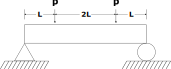
\includegraphics[width=0.6\columnwidth]{q30.png}
        \caption*{}
        \label{fig:q30}
    \end{figure}
    
    \hfill{\brak{\text{GATE IN 2018}}}

    \item In the figure, an RLC load is supplied by a $230$ V, $50$ Hz single phase source. The magnitude of the reactive power \brak{\text{in VAr}} supplied by the source is \underline{\hspace{2cm}}.
    \begin{figure}[H]
        \centering
        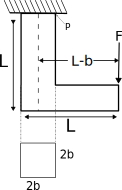
\includegraphics[width=0.5\columnwidth]{q31.png}
        \caption*{}
        \label{fig:q31}
    \end{figure}
    
    \hfill{\brak{\text{GATE IN 2018}}}

    \item In the given circuit, the mesh currents $I_{1}$, $I_{2}$ and $I_{3}$ are
    \begin{figure}[H]
        \centering
        \includegraphics[width=0.4\columnwidth]{q32.png}
        \caption*{}
        \label{fig:q32}
    \end{figure}
    
    \hfill{\brak{\text{GATE IN 2018}}}
    \begin{enumerate}
        \begin{multicols}{2}
            \item $I_{1}=1$ A, $I_{2}=2$ A and $I_{3}=3$ A
            \item $I_{1}=2$ A, $I_{2}=3$ A and $I_{3}=4$ A
            \item $I_{1}=3$ A, $I_{2}=4$ A and $I_{3}=5$ A
            \item $I_{1}=4$ A, $I_{2}=5$ A and $I_{3}=6$ A
        \end{multicols}
    \end{enumerate}
    
    \item The Fourier transform of a signal $x\brak{t}$, denoted by $X\brak{j\omega}$, is shown in the figure. Let $y\brak{t} = x\brak{t} + e^{jt}x\brak{t}$. The value of Fourier transform of $y\brak{t}$ evaluated at the angular frequency $\omega= 0.5$ rad/s is
    \begin{figure}[H]
        \centering
        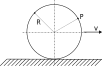
\includegraphics[width=0.5\columnwidth]{q33.png}
        \caption*{}
        \label{fig:q33}
    \end{figure}
    
    \hfill{\brak{\text{GATE IN 2018}}}
    \begin{enumerate}
        \begin{multicols}{4}
            \item $0.5$
            \item $1$
            \item $1.5$
            \item $2.5$
        \end{multicols}
    \end{enumerate}

    \item Let $y[n] = x[n] * h[n]$, where $*$ denotes convolution and $x[n]$ and $h[n]$ are two discrete time sequences. Given that the z-transform of $y[n]$ is $Y\brak{z} = 2 + 3z^{-1} + z^{-2}$, the z-transform of $p[n] = x[n] * h[n-2]$ is
    
    \hfill{\brak{\text{GATE IN 2018}}}
    \begin{enumerate}
        \begin{multicols}{4}
            \item $2 + 3z + z^{-2}$
            \item $3z + z^{-2}$
            \item $2z^2 + 3z + 1$
            \item $2z^{-2} + 3z^{-3} + z^{-4}$
        \end{multicols}
    \end{enumerate}
    
    \item For the sequence $x[n] = \{1, -1, 1, -1\}$, with $n = 0,1,2,3$, the DFT is computed as $X\brak{k} = \sum_{n=0}^{3} x[n]e^{-j\frac{2\pi}{4}nk}$, for $k = 0,1,2,3$. The value of $k$ for which $X\brak{k}$ is not zero is
    
    \hfill{\brak{\text{GATE IN 2018}}}
    \begin{enumerate}
        \begin{multicols}{4}
            \item $0$
            \item $1$
            \item $2$
            \item $3$
        \end{multicols}
    \end{enumerate}
    
    \item Consider the standard negative feedback configuration with $G\brak{s} =\frac{s^2+0.2s+100}{s^2-0.2s+100}$ and $H\brak{s} =\frac{1}{2}$. The number of clockwise encirclements of $\brak{-1,0}$ in the Nyquist plot of the Loop transfer-function $G\brak{s}H\brak{s}$ is \underline{\hspace{2cm}}.
    
    \hfill{\brak{\text{GATE IN 2018}}}

    \item Consider the linear system $\dot{x} = \myvec{-1 & 0\\0 & -2} x$, with initial condition $x\brak{0} = \myvec{1\\1}$. The solution $x\brak{t}$ for this system is
    
    \hfill{\brak{\text{GATE IN 2018}}}
    \begin{enumerate}
        \begin{multicols}{2}
            \item $x\brak{t} = \myvec{e^{-t} & te^{-2t}\\0 & e^{-2t}}\myvec{1\\1}$
            \item $x\brak{t} = \myvec{e^{-t} & 0\\0 & e^{2t}}\myvec{1\\1}$
            \item $x\brak{t} = \myvec{e^{-t} & -t^2e^{-2t}\\0 & e^{-2t}}\myvec{1\\1}$
            \item $x\brak{t} = \myvec{e^{-t} & 0\\0 & e^{-2t}}\myvec{1\\1}$
        \end{multicols}
    \end{enumerate}

    \item Consider a standard negative feedback configuration with $G\brak{s} =\frac{1}{\brak{s+1}\brak{s+2}}$ and $H\brak{s} =\frac{s+\alpha}{s}$. For the closed loop system to have poles on the imaginary axis, the value of $\alpha$ should be equal to \brak{\text{up to one decimal place}} \underline{\hspace{2cm}}.
    
    \hfill{\brak{\text{GATE IN 2018}}}

    \item Unit step response of a linear time invariant \brak{LTI} system is given by $y\brak{t} = \brak{1 - e^{-2t}}u\brak{t}$. Assuming zero initial condition, the transfer function of the system is
    
    \hfill{\brak{\text{GATE IN 2018}}}
    \begin{enumerate}
        \begin{multicols}{4}
            \item $\frac{1}{s+1}$
            \item $\frac{2}{\brak{s+1}\brak{s+2}}$
            \item $\frac{1}{s+2}$
            \item $\frac{2}{s+2}$
        \end{multicols}
    \end{enumerate}

    \item In the given relaxation oscillator, the opamps and the zener diodes are ideal. The frequency \brak{\text{in kHz}} of the square wave output vo is \underline{\hspace{2cm}}.
    \begin{figure}[H]
        \centering
        \includegraphics[width=0.7\columnwidth]{q40.png}
        \caption*{}
        \label{fig:q40}
    \end{figure}
    
    \hfill{\brak{\text{GATE IN 2018}}}

    \item An opamp that is powered from a $\pm 5$V supply is used to build a non-inverting amplifier having a gain of $15$. The slew rate of the opamp is $0.5\times10^6$ V/s. For a sinusoidal input with amplitude of $0.3$ V, the maximum frequency \brak{\text{in kHz}} up to which it can be operated without any distortion is \brak{\text{up to one decimal place}} \underline{\hspace{2cm}}.
    
    \hfill{\brak{\text{GATE IN 2018}}}

    \item The circuit given uses ideal opamps. The current I \brak{\text{in }\mu\text{A}} drawn from the source $v_s$ is \\ \brak{\text{up to two decimal places}} \underline{\hspace{2cm}}.
    \begin{figure}[H]
        \centering
        \includegraphics[width=0.5\columnwidth]{q42.png}
        \caption*{}
        \label{fig:q42}
    \end{figure}
    
    \hfill{\brak{\text{GATE IN 2018}}}

    \item The product of sum expression of a Boolean function $F\brak{A, B, C}$ of three variables is given by
    \begin{align*}
    F\brak{A, B, C} = \brak{ A + B + \bar{C} } \cdot \brak{A + \bar{B} + \bar{C} } \cdot \brak{ \bar{A} + B + C } \cdot \brak{ \bar{A} + \bar{B} + \bar{C} }
    \end{align*}
    The canonical sum of product expression of $F\brak{A, B, C}$ is given by
    
    \hfill{\brak{\text{GATE IN 2018}}}
    \begin{enumerate}
        \item $\bar{A}\bar{B}C + \bar{A}B C + A\bar{B}\bar{C} + A B C$
        \item $\bar{A}\bar{B}\bar{C} + \bar{A}B\bar{C} + A\bar{B}C + AB\bar{C}$
        \item $A B \bar{C} + A \bar{B} \bar{C} + \bar{A} B C + \bar{A} \bar{B} \bar{C}$
        \item $\bar{A}\bar{B}\bar{C} + \bar{A}B C + A B \bar{C} + A B C$
    \end{enumerate}

    \item A 2-bit synchronous counter using two J-K flip flops is shown. The expressions for the inputs to the J-K flip flops are also shown in the figure. The output sequence of the counter starting from $Q_1Q_2 = 00$ is
    \begin{figure}[H]
        \centering
        \includegraphics[width=0.6\columnwidth]{q44.png}
        \caption*{}
        \label{fig:q44}
    \end{figure}
    
    \hfill{\brak{\text{GATE IN 2018}}}
    \begin{enumerate}
        \item $00 \to 11 \to 10 \to 01 \to 00 \cdots$
        \item $00 \to 01 \to 10 \to 11 \to 00 \cdots$
        \item $00 \to 01 \to 11 \to 10 \to 00 \cdots$
        \item $00 \to 10 \to 11 \to 01 \to 00 \cdots$
    \end{enumerate}

    \item A portion of an assembly language program written for an 8-bit microprocessor is given below along with explanations. The code is intended to introduce a software time delay. The processor is driven by a 5 MHz clock. The time delay \brak{\text{in } \mu\text{s}} introduced by the program is \underline{\hspace{2cm}}.
    \begin{verbatim}
 MVI B, 64H ; Move immediate the given byte into register B. 
            ; Takes 7 clock periods.
 LOOP:DCR B ; Decrement register B. Affects Flags. 
            ; Takes 4 clock periods.
 JNZ LOOP   ; Jump to address with Label LOOP if zero flag is not set.
            ; Takes 10 clock periods when jump is performed and 
            ; 7 clock periods when jump is not performed.
    \end{verbatim}
    
    \hfill{\brak{\text{GATE IN 2018}}}
    
    \item The Boolean function $F\brak{ X, Y}$ realized by the given circuit is
    \begin{figure}[H]
        \centering
        \includegraphics[width=0.6\columnwidth]{q46.png}
        \caption*{}
        \label{fig:q46}
    \end{figure}
    
    \hfill{\brak{\text{GATE IN 2018}}}
    \begin{enumerate}
        \begin{multicols}{4}
            \item $\bar{X}Y + X\bar{Y}$
            \item $\bar{X}\bar{Y} + XY$
            \item $X + Y$
            \item $\bar{X} \cdot \bar{Y}$
        \end{multicols}
    \end{enumerate}

    \item The voltage and current drawn by a resistive load are measured with a 300 V voltmeter of accuracy $\pm 1\%$ of full scale and a 5 A ammeter of accuracy $\pm 0.5\%$ of full scale. The readings obtained are 200 V and 2.5 A. The limiting error \brak{\text{in }\%} in computing the load resistance is \brak{\text{up to two decimal places}} \underline{\hspace{2cm}}.
    
    \hfill{\brak{\text{GATE IN 2018}}}

    \item A high Q coil having distributed \brak{self} capacitance is tested with a Q-meter. First resonance at $\omega_1 = 10^6$rad/s is obtained with a capacitance of 990 pF. The second resonance at $\omega_2 = 2 \times 10^6$rad/s is obtained with a 240 pF capacitance. The value of the inductance \brak{\text{in mH}} of the coil is \brak{\text{up to one decimal place}} \underline{\hspace{2cm}}.
    
    \hfill{\brak{\text{GATE IN 2018}}}

    \item The inductance of a coil is measured using the bridge shown in the figure. Balance \brak{D = 0} is obtained with $C_1 = 1$ nF, $R_1 = 2.2$ M$\ohm$, $R_2 = 22.2$ k$\ohm$, $R_4 = 10$ k$\ohm$. The value of the inductance $L_x$ \brak{\text{in mH}} is \underline{\hspace{2cm}}.
    \begin{figure}[H]
        \centering
        \includegraphics[width=0.5\columnwidth]{q49.png}
        \caption*{}
        \label{fig:q49}
    \end{figure}
    
    \hfill{\brak{\text{GATE IN 2018}}}

    \item The average velocity v of flow of clear water in a 100 cm \brak{\text{inner}} diameter tube is measured using the ultrasonic flow meter as shown in the figure. The angle $\theta$ is $45\degree$. The measured transit times are $t_1 = 0.9950$ ms and $t_2 = 1.0000$ ms. The velocity v \brak{\text{in m/s}} in the pipe is \brak{\text{up to one decimal place}} \underline{\hspace{2cm}}.
    \begin{figure}[H]
        \centering
        \includegraphics[width=0.6\columnwidth]{q50.png}
        \caption*{}
        \label{fig:q50}
    \end{figure}
    
    \hfill{\brak{\text{GATE IN 2018}}}
    
    \item A $1000~\ohm$ strain gage \brak{R_g} has a gage factor of $2.5$. It is connected in the bridge as shown in figure. The strain gage is subjected with a positive strain of $400~\mu$m/m. The output $V_o$ \brak{\text{in mV}} of the bridge is \brak{\text{up to two decimal places}} \underline{\hspace{2cm}}.
    \begin{figure}[H]
        \centering
        \includegraphics[width=0.8\columnwidth]{q51.png}
        \caption*{}
        \label{fig:q51}
    \end{figure}
    
    \hfill{\brak{\text{GATE IN 2018}}}

    \item Assuming ideal opamp, the RMS voltage \brak{\text{in mV}} in the output Vo only due to the 230 V, 50 Hz interference is \brak{\text{up to one decimal place}} \underline{\hspace{2cm}}.
    \begin{figure}[H]
        \centering
        \includegraphics[width=0.5\columnwidth]{q52.png}
        \caption*{}
        \label{fig:q52}
    \end{figure}
    
    \hfill{\brak{\text{GATE IN 2018}}}

    \item The sampling rate for Compact Discs \brak{CDs} is $44,000$ samples/s. If the samples are quantized to $256$ levels and binary coded, the corresponding bit rate \brak{\text{in bits per second}} is \underline{\hspace{2cm}}.
    
    \hfill{\brak{\text{GATE IN 2018}}}

    \item A Michelson Interferometer using a laser source of wavelength $\lambda_0 = 500$ nm, with both the mirrors \brak{M_1\& M_2} fixed and positioned equidistant from the splitter/combiner is shown in the figure. When a dielectric plate of refractive index $n = 1.5$, of thickness $t$, is placed in front of the mirror $M_2$, a dark fringe is observed on the detector. When the dielectric plate is removed without changing the position of the mirrors $M_1\& M_2$, a bright fringe is observed on the detector. The minimum thickness $t$ \brak{\text{in nm}} of the dielectric is \underline{\hspace{2cm}}.
    \begin{figure}[H]
        \centering
        \includegraphics[width=0.5\columnwidth]{q54.png}
        \caption*{}
        \label{fig:q54}
    \end{figure}
    
    \hfill{\brak{\text{GATE IN 2018}}}

    \item A multi-mode optical fiber with a large core diameter has a core refractive index $n_1 = 1.5$ and cladding refractive index $n_2 = 1.4142$. The maximum value of $\theta_A$ \brak{\text{in degrees}} for which the incident light from air will be guided in the optical fiber is $\pm$\underline{\hspace{2cm}}.
    \begin{figure}[H]
        \centering
        \includegraphics[width=0.7\columnwidth]{q55.png}
        \caption*{}
        \label{fig:q55}
    \end{figure}
    
    \hfill{\brak{\text{GATE IN 2018}}}

\end{enumerate}
\end{document}
